\documentclass[aps,prl,twocolumn,superscriptaddress,10pt]{revtex4-1}  % for review and submission
%\documentclass[aps,twocolumn,floatfix,prl,10pt]{revtex4-1}
%\documentclass[letterpaper,10pt,prl,twocolumn,aps]{revtex4-1}
%\documentclass[aps,preprint,floatfix,prl]{revtex4-1}
\usepackage{amsmath}
\usepackage{amsfonts}
\usepackage{amssymb}
\usepackage{graphicx}
\usepackage{booktabs}
\usepackage{color}
\usepackage{longtable}
\usepackage{array}
\usepackage{amssymb}
\usepackage[usenames,dvipsnames,svgnames,table]{xcolor}

\graphicspath{ {images/}{images/Growth_Rate_Cont_Plots/} }
\newcommand{\bn}{{\boldsymbol{\hat{n}}}}
\newcommand{\bt}{{\boldsymbol{\hat{t}}}}
\newcommand{\bu}{\mathbf{u}}
\newcommand{\grad}{\mathbf{\nabla}}
\newcommand{\del}{\partial}
\newcommand{\hg}{h_g}
\newcommand{\Rey}{\text{R}}
\newcommand{\Ndg}{\tilde{N}_g}
\newcommand{\monami}{\textit{monami}}
\newcommand{\ubl}{u_\text{bl}}
\definecolor{tableShade}{gray}{0.8}

\begin{document}
\title{\textit{Monami} as an oscillatory hydrodynamic instability in a submerged sea grass bed}
\author{Ravi Singh}
\affiliation{Brown University, Providence RI 02912 USA}
\author{L. Mahadevan}
\affiliation{Harvard University, Cambridge MA 02138 USA}
\author{M. M. Bandi}
\affiliation{OIST Graduate University, Okinawa 904-0495, Japan}
\author{Amala Mahadevan}
\affiliation{Woods Hole Oceanographic Institution, Woods Hole MA 02543 USA}
\author{Shreyas Mandre}
\affiliation{Brown University, Providence RI 02912 USA}

\begin{abstract}
The onset of \monami ~-- the synchronous waving of sea grass beds driven by a steady flow -- is modeled as a linear instability of the steady flow. Our model treats the drag exerted by the grass in establishing the steady flow profile, and in damping out perturbations to it. This damping leads to a finite threshold flow for the instability, which agrees with experimental observations. This role of vegetation drag differentiates our mechanism from the previous hypothesis that the Kelvin-Helmholtz instability underlies \monami.
\end{abstract}

\maketitle
Sea grasses exhibit a rich set of dynamical behavior due to their collective interaction with both steady and oscillatory flows.  
The hydrodynamic processes resulting from this behavior influence a number of environmental processes such as transport of sediments, contaminants, dissolved oxygen, plant growth, and biomass production  \cite{Fonseca87,Grizzle96,Nepf99,Nepf2012}. 
One such response of these grass beds to steady currents is the formation of coherent large amplitude oscillations, known as \monami ~\cite{AckermanOkubo93}.  
In this letter, we provide a hydrodynamic mechanism for the onset of these coherent oscillations.
\newline
Current explanations of \monami ~invoke the existence of a free shear layer at the top of the grass bed (henceforth called grass top) due to vegetation drag  \cite{Ghisal02,Raupach96}. 
Its instability, through a mechanism similar to the Kelvin-Helmholtz instability, is thought to lead to coherent eddies over the grass bed, and drive large amplitude synchronous oscillations.
This model has been applied successfully to ...!
\newline
% While the shear layer model appears to predict the frequency of \monami ~consistent with experimental observations, s
However, several aspects of the shear layer model remain unsatisfactory: 
(i)   The velocity profile of the free shear layer is assumed \textit{ad hoc} to be piecewise linear \cite{Delangre06} or hyperbolic tangent \cite{Ghisal02,Raupach96}. 
(ii)  The role of drag in damping the perturbations to the shear profile is sometimes ignored \cite{Raupach96}. 
% (i) While the free shear layer is established due to the vegetation drag, linear stability analysis \cite{Raupach96} does not account for this, rendering this explanation inconsistent (however, see ref. \cite{White07}). 
(iii) Observations in the lab \cite{Ghisal02} and the field \cite{Grizzle96} indicate the existence of a threshold flow speed below which \monami ~is not observed. No existing theory has explained this threshold condition. 
(iv)  The thickness of the free shear layer is in many cases comparable to the unvegetated layer thickness, and therefore inconsistent with the definition of the free shear layer.
Here we present a mathematical model for the linear instability that accounts correctly for these effects, while also explaining lab experiments and field observations.
\newline
Although \monami ~is manifest in the motion of the grass, the drag exerted by the grass bed on the flow is central to the hypothesized instability. 
The instability and the resulting flow structures persist in lab experiments even when flexible grass mimics are replaced by rigid dowels \cite{Ghisal02}. 
% Therefore, we consider the grass bed to be rigid to probe the essential features of the instability. 
% Therefore, assuming that the restoring force of buoyancy is sufficiently strong, we neglect the motion of the grass blades in this analysis.
% Therefore we neglect the motion of the grass blades in this analysis, assuming that a small deviation from its equilibrium position generates sufficient restoring force to balance the fluid drag. 
Therefore, to develop the essential mathematical model, we assume the vegetation to be rigid, and verify it \textit{a posteriori}.
% Indeed, a more detailed calculation modeling terrestrial grass demonstrated \cite{Delangre06} that when the timescale of the instability is well-separated from the period of natural oscillations of the grass bed, the flow instability is similar to the instability of a shear layer. 
\begin{figure}
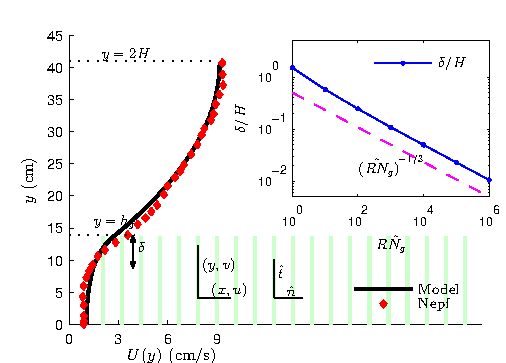
\includegraphics[scale=1]{Grass_Base_Nepf_shear}
\caption{Schematic setup and comparison of a steady flow profile from the experiments by Ghisalberti and Nepf \cite{Nepf04} (Case-I from Table-1 with 1250 plants/m$^2$, 
plant height = 13.7$\pm 0.2$ cm and blade width of 0.64 cm)
 and its approximation with $U_0=7.28$ cm/s and $\delta = 5.02$ cm in our model. The grass extends up to $y=h_g$ in the water column of depth $2H$. 
The steady velocity profile can be decomposed into three regions, (i) A parabolic profile in the unvegetated region, (ii) a uniform profile deep within the vegetation, and (iii) a boundary layer of thickness $\delta$ near the grass top. 
The dependence of the boundary layer thickness (estimated as $|U/U_y|$ at $y=\hg$ from the numerical solution of \eqref{base_equ}) on the vegetation density parameter $\Rey \Ndg$ is shown in the inset.}
\label{basicflow}
\end{figure}
\begin{figure}
\begin{center}
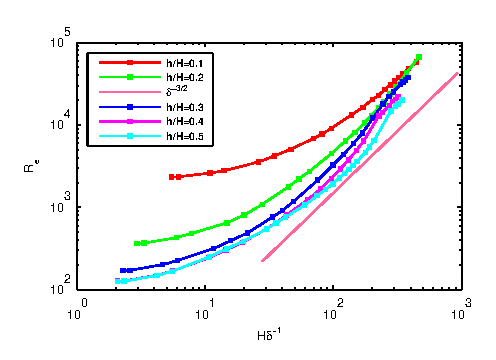
\includegraphics[]{Critical_Re_vs_delta_noshear} \\
\vspace{-6mm} \hspace{-3mm}
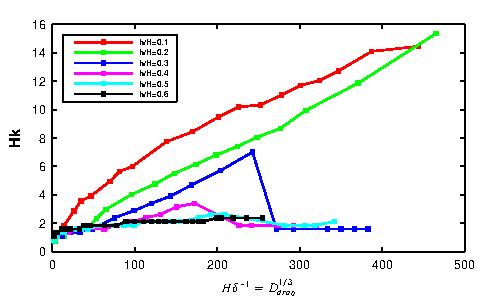
\includegraphics[]{K_vs_shear_width_noshear}
\end{center}
\caption{Critical Reynolds number (top) and the corresponding marginally stable wave number (bottom) for different submergence ratio as a function of vegetation density parametrized by the boundary layer thickness. 
Parameters estimated from experiments reported by Ghisalberti and Nepf \cite{Ghisal02} to exhibit or suppress synchronous waving are also included in the top panel. 
Inset compares experimental observations of the experimentally measured dominant frequency $f_o$ (in Hz) with the predictions from the solution of eq.~\eqref{Orr-somerfield}. 
The experimental data in the inset is obtained from publications by Ghisalberti and Nepf \cite{Ghisal02} and Vivoni \cite{Vivoni98}. 
In order to estimate the $\Rey$ for these experiments, a representative value of $\mu=0.1$ Pa~s was assumed.}
\label{Re_vs_delta}
\end{figure}

% We use a mean field model for the coupling between the flow and the vegetation. 
The drag exerted by the vegetation on the flow is approximated by a continuous body force $\mathbf{f}=-N_g\mathbf{f_d}$,  where $\mathbf{f_{d}}$ is the drag force per unit length of the grass blade, and $N_g$ the grass blade number density per unit horizontal area \cite{Vivoni98,Nepf99,Ghisal02,Delangre04,Delangre06}. 
This drag enters the governing equations of continuity and momentum balance, written as 
\begin{equation}
\quad \grad\cdot\bu = 0,\hspace{3mm} \rho \left(\bu_{t}+\bu.\grad\bu \right) = -\grad p+\mu\grad^{2}\bu +\mathbf{f}+\rho\mathbf{g}
\label{navier-stokes}
\end{equation}
where $\rho$ is the fluid density, $\mathbf{u}$ the velocity, 
$p$ the pressure, $\mu$ the eddy viscosity (the flow is turbulent) and $\mathbf{g}$ the acceleration due to gravity. 
The Reynolds number of the flow based on the scale of the grass blade is $O(10^2-10^3)$; therefore the form drag on the vegetation dominates over the skin-friction. 
We model it as 
$\mathbf{f_{d}}=C_N \rho u_{N}^{2}d\bn$, 
where $d$ is the average width of grass blade projected in the flow direction, $C_{N}$ the drag coefficient, and $u_{N}$ and $\bn$ are the velocity component and unit vector normal to the grass (see fig.~\ref{basicflow} for a schematic). 
In the field, both $C_N$ and $N_g$ vary with position, but we do not expect these variations to be central to the instability mechanism, and therefore take $C_N$ and $N_g$ to be constants. 
Based on previous experiments \cite{Vivoni98}, we take $C_N \approx 1$.
\newline
\begin{figure*}
\begin{tabular}{cccc}
{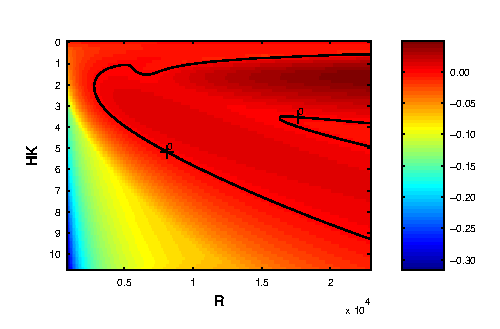
\includegraphics[scale = 0.85]{Set4_dens28_imgsc}} &
%{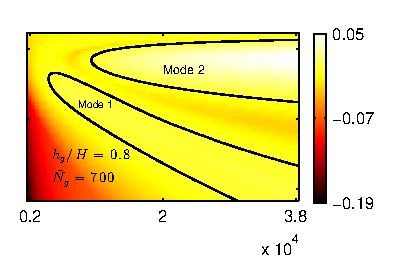
\includegraphics[scale = 0.67]{Set4_dens30_imgsc}} &
{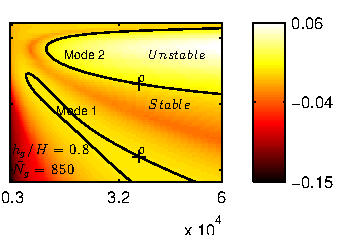
\includegraphics[scale = 0.85]{Set4_dens32_imgsc}} &
{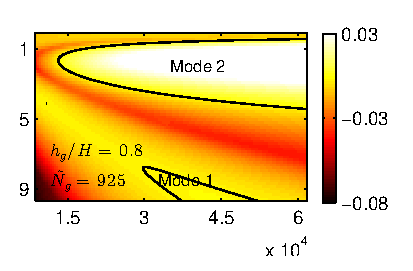
\includegraphics[scale = 0.85]{Set4_dens34_imgsc}} \\
{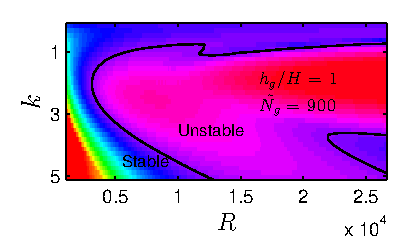
\includegraphics[scale = 0.85]{Set5_dens38_imgsc}} &
%{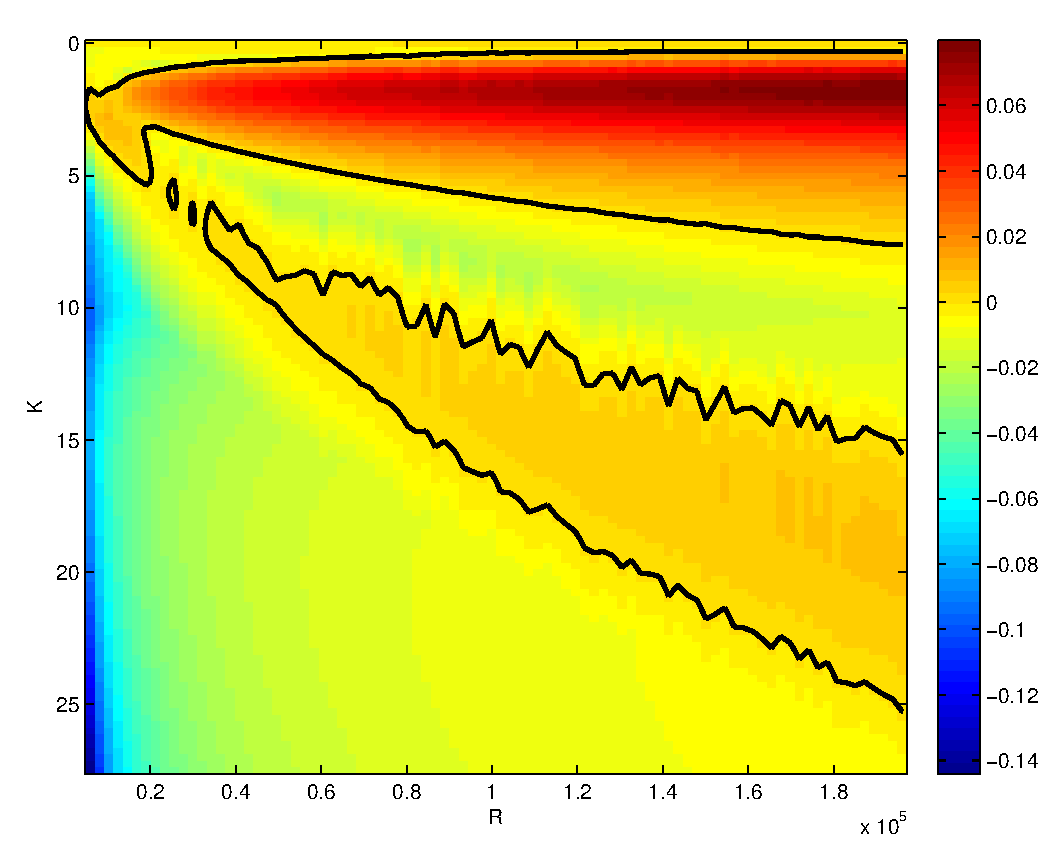
\includegraphics[scale = 0.67]{Set5_dens40_imgsc}} &
{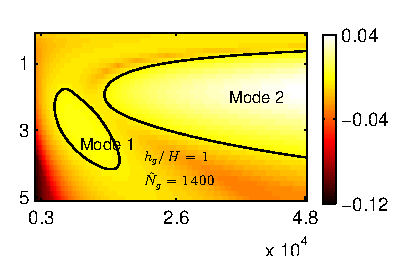
\includegraphics[scale = 0.85]{Set5_dens42_imgsc}} &
{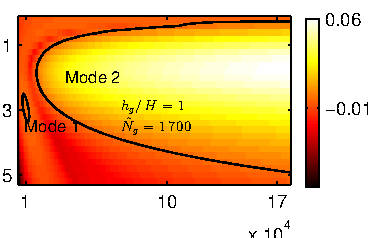
\includegraphics[scale = 0.85]{Set5_dens46_imgsc}} \\
%{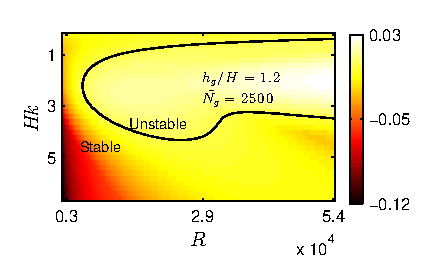
\includegraphics[scale = 0.67]{Set6_dens32_imgsc}} &
%{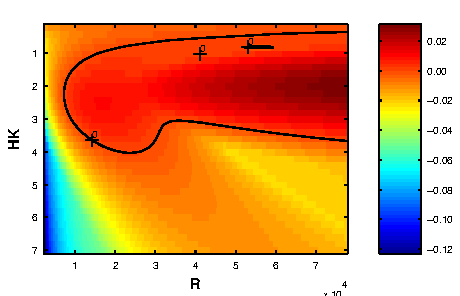
\includegraphics[scale = 0.67]{Set6_dens34_imgsc}} &
%{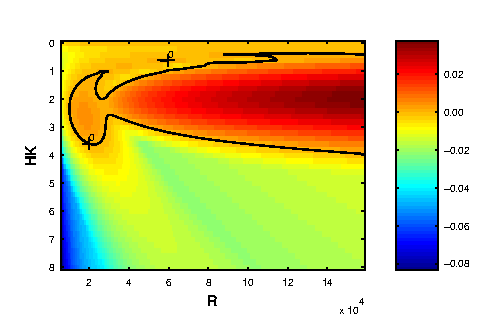
\includegraphics[scale = 0.67]{Set6_dens36_imgsc}} &
%{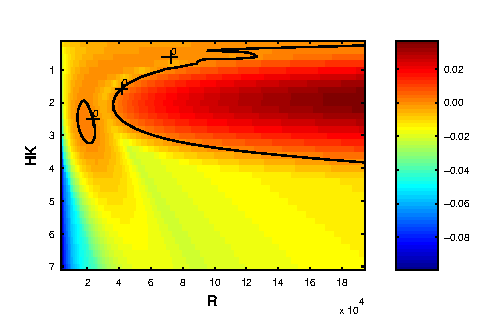
\includegraphics[scale = 0.67]{Set6_dens38_imgsc}}
\end{tabular}
\caption{$Re(\sigma)$ as function of wavenumber and Reynolds number for a specified vegetation number density $\Ndg$ along with the neutral curve ($Re(\sigma)$=0), for parameters shown in the corresponding panel.  
As $\Ndg \propto N_g$ increases, the unstable region splits into two labeled as ``Mode 1'' and ``Mode 2''. 
For $\Ndg$ below a critical value, the Mode 1 sets the threshold $\Rey$ whereas above the critical $\Ndg$ onset is determined by Mode 2.}
\label{K_Re_sigma_set3}
\end{figure*}
We first calculate the fully developed steady flow $\bu = U(y)\boldsymbol{\hat{x}}$ driven by constant pressure gradient $dP/dx$ as a solution of eq.~\eqref{navier-stokes}. 
Such a flow satisfies 
\begin{equation}
 -\frac{dP}{dx}+\mu U''(y) +S(y) \rho C_N d N_gU^2=0
\label{base_equ}
\end{equation}
where $S(y)=1$ in the grass bed ($0<y<\hg$) and $S(y)=0$ above it ($\hg< y< 2H$). 
Eq. \eqref{base_equ} is solved subject to no shear at the boundaries, i.e., $U'(0) = U'(2H) = 0$.
The former arises because, in the case of dense vegetation, the shear stress exerted by the bottom surface is expected to be negligible compared to the vegetation drag. 
This expectations is verified by a comparison, shown in fig.~\ref{basicflow}, of the steady flow profile from the solution of eq.~\eqref{base_equ} with experimental measurements.
The profile $U(y)$ has three distinct regions.
Within vegetation, it is approximately uniform with $ U(y) \approx U_g = \sqrt{\frac{dP/dx}{\rho C_N dN_g}}$, arising from the balance between drag and pressure gradient. 
Outside the vegetation, the velocity has a simple parabolic profile due to the balance between viscous forces and the pressure gradient. 
At the grass top, continuity of shear stresses results in a boundary layer of thickness $\delta$. 
Because this boundary layer develops from purely local dynamics, independent of the influence of the boundaries, and we identify to be analogous to the free shear layer \cite{Ghisal02} in the previous explanation of \monami.
Denoting $\ubl$ to be the velocity scale in boundary layer, and $U_0 = {(dP/dx)~H^2}/{\mu}$ the velocity scale in the unvegetated region, the balance of the viscous forces and the vegetation drag implies $(\mu \ubl/\delta^2 \sim \rho C_N d N_g \ubl^2)$, and the continuity of shear stress across the grass top implies $(\ubl/\delta \sim U_0/H)$,  
Solving for $\delta$ yields $\delta=(\Rey\tilde{N_g})^{-1/3}H$, where $\Ndg = \left(C_N d H N_g\right)$ is the vegetation frontal area per bed area, and $\Rey=\rho U_0 H/\mu$ is the Reynolds number of the flow. 
This dependence of the boundary layer thickness on the vegetation density $N_g$, verified in fig.~\ref{basicflow}, gives us a way to systematically investigate its effect on the instability mechanism.
The asymptotic regime of a thin boundary layer is expected to hold for $\Rey \Ndg \gtrsim 100$.
% ; minor departures from this scaling can be seen in the inset of fig.~\ref{basicflow}.
\newline
To understand the evolution of small perturbations to the steady flow profile, we substitute $\bu = (U+\tilde{u}, \tilde{v})$, $p=P+\tilde{p}$ in eq.~\eqref{navier-stokes} and expand to linear order to obtain (after dropping the tilde decoration)
\begin{equation}
\begin{split}
\rho(u_t+U u_x+vU_y) &= -p_x+ {\mu}\nabla^2u-2S\rho C_{N}dN_{g}Uu, \\
\rho(v_t+ Uv_x) &= -p_y+ {\mu}\nabla^2v, \hspace{0.3cm} \nabla\cdot\bu=0.
\end{split}
\end{equation}
These equations can be non-dimensionalized using half channel height $H$, velocity $U_0$, and the associated advection time $H/U_0$, leading to three non-dimensional parameters, \textit{viz.} $\Rey$, $\Ndg$, and the submergence ratio of the vegetation $h_g/H$. 
We also use $\delta/H$ in lieu of $\Ndg$ to parametrize the vegetation density and help elucidate the mechanism of the instability. 
With these scalings, and using a stream function $\psi$ with $u = \psi_{y}, v= -\psi_x$ to satisfy mass balance, we seek a wave solution of 
the form $\left(u,v,\psi \right)= \left(\hat u(y), \hat v(y), \hat\phi(y) \right)e^{ikx+\sigma t}$ to  obtain a modified Orr-Sommerfield equation 
\begin{equation}
\begin{split}
\left(D^2 -k^{2} \right)^2\phi &= \Rey \left[ \left({\sigma}+ikU\right) \left(D^2-k^2\right) -ikU_{yy}\right]\phi \\
&+D\left(2R \Ndg S U D \phi\right),
\label{Orr-somerfield}
\end{split}
\end{equation}
where $D=d/dy$, and subject to the boundary conditions $D\phi = D^2\phi = 0$ at $y=0$ and $y=2$. 
The growth rate $\sigma$ for a given wave number $k$ is the eigenvalue that allows a non-trivial solution $\phi$ of eq. \eqref{Orr-somerfield}.

A threshold in $\Rey$ of $O(100)$, above which the flow is unstable (Re$(\sigma)>0$) for at least one $k$, emerges from the 
solution of eq.~\eqref{Orr-somerfield}. The dependence of this threshold $\Rey$, and the corresponding marginally stable wavenumber $k$, on $\delta/H$ and $\hg/H$ is shown 
in fig.~\ref{Re_vs_delta}, and is found to compare well with experimental observations \cite{Ghisal02}.
The threshold Reynolds number increases with the vegetation density, indicating a competition between the 
destabilizing shear in the flow, and the stabilizing effect of damping due to vegetation drag.
A similar conclusion was presented \cite{White07} for flow around an emergent (i.e., $\hg>2H$) sea grass patch, but by assuming $U(y)$ to be a tanh-profile \textit{ad hoc}, and neglecting the viscous term.
Previous linear stability calculations for terrestrial grass have not reported a threshold flow condition 
either due to the exclusion of the vegetation drag in their model \cite{Raupach96}, or because of the \textit{ad hoc}
assumptions about the mean velocity profile \cite{Raupach96,Delangre06}. 

Comparison of frequency (Im$(\sigma)$) of the fastest growing mode with that of experimental observations of frequencies in
the lab scale experiments, for cases where the vegetation was sufficiently dense to be modeled by a continuum drag field, is also shown in the inset in fig.~\ref{Re_vs_delta}b. 
The observed frequencies are associated with the peaks in velocity spectra, frequency of \monami ~and frequency of 
vortex passage \cite{Ghisal02}, and compare well with the predicted frequencies. The experimentally observed \monami ~wavelengths are not available for comparison.

\begin{table*}
\rowcolors{3}{tableShade}{white}  %% start alternating shades from 3rd row
\renewcommand{\arraystretch}{1.4}
 \begin{tabular}{l|c|c|c}
			& Kelvin-Helmholtz 				& Mode 1 		& Mode 2 \\ \hline
 Base velocity profile 	& $U(y) = U_0 \tanh(y/\delta)$			& \multicolumn{2}{c}{Equation \eqref{base_equ}} \\
 Domain 		& $-\infty < y < \infty$			& \multicolumn{2}{c}{$-1<y<1$} \\
 Inflection point	& exists at $y=0$				& \multicolumn{2}{c}{$U''(y)$ discontinuous at $y=\hg$} \\
 Shear layer thickness	& $\delta$					& \multicolumn{2}{c}{$\delta \sim  H\left(\Rey \Ndg \right)^{-1/3}$} \\
 Linearized dynamics	& $\left(\sigma+ikU\right) \left(D^2-k^2\right)\phi =  ikU_{yy}\phi$		& \multicolumn{2}{c}{Equation \eqref{Orr-somerfield}} \\
 Dense grass limit &  & Equation \eqref{eqn:mode1asymp} & Equation \eqref{eqn:mode2asymp}  \\
 Critical parameters	& none						& $\Rey \propto \Ndg^{1/2}$ 	& $\Rey \propto \Ndg$ \\
 Most unstable $k$ as $\delta \to 0$	& $\propto H/\delta$		& $\propto H/\delta$	& $O(1)$ \\
 Mode localized?	& yes, near $y=0$				& ~~yes, near $y=\hg$~~			& ~~no, spans water column~~
 \end{tabular}
 \caption{Comparison between Kelvin-Helmholtz instability and the two modes resulting from solution of \ref{Orr-somerfield}.}
 \label{tab:comparison}
\end{table*}
To better understand the mechanism of waving and the origin of the threshold, we consider the behavior of the instability as a function of the vegetation drag characterized by $\Ndg$.
The fastest growing wavenumber first increases proportional to $H/\delta$, but at a critical vegetation density discontinuously jumps and remains $O(1)$ (see fig.~\ref{Re_vs_delta}). 
To aid in explaining the behavior, we show heat maps of Re$(\sigma)$ as a function of $\Rey$ and $k$, for different $\hg/H$ and $\Ndg$ in fig.~\ref{K_Re_sigma_set3}. 
The lowest $\Rey$ on the neutral curve sets the threshold. 
We observe that as $\Ndg$ increases, the unstable region splits into two. We refer to the unstable region with the higher $k$ as ``Mode 1'', and the one with the lower $k$ as ``Mode 2''. 
The unstable region for Mode 1, depending on $\hg/H$ either recedes to higher $\Rey$ or shrinks to zero size, as the vegetation density increases, causing the most unstable mode to transition discontinuously.

The distinct asymptotic behavior of the two modes as $\Ndg \gg 1$ allows us to understand the mechanism of the instability. 
Mode 1 asymptotically localizes to the boundary layer near the top of the vegetation, and exhibits an asymptotic behavior with $k \sim O(H/\delta)$, and $\Rey \sim (H/\delta)$ (or $\Rey \propto {\Ndg}^{1/2}$) at the threshold. 
This limit can be understood through asymptotically estimating the sizes of the terms in eq.~\eqref{Orr-somerfield} using $D\sim \delta^{-1}$, $\sigma \sim \delta^{-1}$, and $U\sim \delta$; the magnitude of the advection term is $\Rey/\delta^3 \sim \Rey^2 \Ndg $, and the viscous term (or the vegetation drag term, which is found to scale identically) in the boundary layer is $\delta^{-4} \sim (\Rey \Ndg)^{4/3}$. 
The terms balance when $\Rey \sim H/\delta$ (or $\Rey \sim {\Ndg}^{1/2}$) leading to a simplification of eq.~\eqref{Orr-somerfield} as
\begin{align}
(D^2-k^2)^2 \phi- 2 \Rey \Ndg D( SUD\phi) = \sigma \Rey (D^2-k^2)\phi,
\label{eqn:mode1asymp}
\end{align} 
in a region of thickness O($\delta$) near $y=\hg$.
Since the relative magnitude of the terms on the r.h.s. to those on the l.h.s. of this equation is $\Rey/\Ndg^{1/2}$, we expect identical asymptotic behavior for fixed $\Rey/\Ndg^{1/2}$. Therefore the threshold obtained for Mode 1 is $\Rey \propto \Ndg^{1/2}$ (or $\Rey \propto H/\delta$) explaining the numerically observed asymptote (see fig.~\ref{Re_vs_delta}). 
This analysis also concludes that the mode structure is self-similar over the length scale $\delta$ for fixed $\Rey/\Ndg^{1/2}$; the verification of this expectation is shown in fig.~\ref{Asymptotic_mode}, supporting this argument.

On the other hand, the threshold condition for Mode 2 is numerically observed to be $\Rey \propto ({\delta}/{H})^{-3/2}$ (or $\Rey \propto \Ndg$) for $k\sim O(1)$, shown in fig.~\ref{Re_vs_delta}, which can be understood by an asymptotic scaling analysis of eq.~\eqref{Orr-somerfield} by assuming $\Rey \gg 1$ but fixed $\Rey/\Ndg \sim O(1)$.
Note that for large $\Ndg$, the non-dimensional steady flow velocity inside the vegetation is $U_g \sim (\Rey \Ndg)^{-1/2}$. 
This estimate simplifies eq.~\eqref{Orr-somerfield} to 
\begin{align}
\begin{split}
\sigma\left(D^2-k^2\right)\phi = -2{(\Ndg/\Rey)^{1/2}}D^2\phi,  \quad &\text{ for $y<\hg$}  \\
\left(\sigma+ikU\right) \left(D^2-k^2\right)\phi =  ikU_{yy}\phi, \quad &\text{ for $y>\hg$}.
\end{split}
\label{eqn:mode2asymp}
\end{align}
\begin{figure}
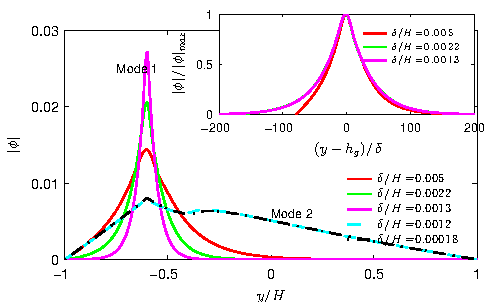
\includegraphics[]{Asymptotic_noshear}
\caption{Plot of mode shape $|\phi|$ for different shear layer thickness in limit of small shear layer thickness for representative values of vegetation density. 
Mode 1 is shown in solid and Mode 2 is shown in dashed. The parameters Mode 2 shapes are chosen such that $\Rey \gg 1$, $\Ndg \gg 1$ (specified in terms of $\delta/H$) but $\Rey/\Ndg = O(1)$. 
The mode shapes approach each other for these small values of $\delta/H$ indicating that the large vegetation density asymptote is reached. Mode 1 shapes appear self-similar in shape as $\delta\to 0$, 
and are compared to each other on a rescaled coordinate in the inset. 
Inset shows $|\phi|$ for Mode 1 as a function of $(y-\hg)/\delta$. The modes approach a universal shape, indicating that an asymptotic limit has been reached. 
The limit is not yet reached for the case $\delta/H = 0.005$ due to the influence of bottom boundary; the vegetation height in this case is comparable to the boundary layer thickness.}
\label{Asymptotic_mode}
\end{figure}
Since $\Rey/\Ndg$ is the only remaining parameter, the mode shape would converge in the aforementioned limit, in agreement with our numerical results for Mode 2 shown in fig.~\ref{Asymptotic_mode}. 
We interpret Mode 2 as the instability of an inviscid flow, with the vegetation modeled by a continuum drag field, and for which the boundary layer near the top of the vegetation plays no role. The only remaining parameter $\Rey/\Ndg$ 
sets the threshold, leading to the asymptotic behavior $\Rey \propto \Ndg$ (or $\Rey \sim ({\delta}/{H})^{-3/2}$).
%On the other hand, Mode 1 asymptotically localizes to the boundary layer near the grass tip, and exhibits a different asymptotic behavior with $k \sim O(H/\delta)$, and $\Rey \sim (H/\delta)$ (or $\Rey \propto {\Ndg}^{1/2}$) at the threshold. 

Table \ref{tab:comparison} compares the two modes to each other, and to the Kelvin-Helmholtz instability. 
Because Mode 1 eigenfunction is localized over a length scale $\delta$, it may be interpreted as the instability of the flow in the boundary layer, whereas Mode 2 may be understood as the instability on the scale of the water column. 
Mode 1 appears to be closely related to the Kelvin Helmholtz mechanism, whereas Mode 2 arises purely from the interaction between the unvegetated water column and the flow through the vegetation. 
Vegetation drag plays a dominant role in the mechanism for both the modes, which distinguishes our analysis from the traditional Kelvin-Helmholtz instability. 
The appearance of vegetation drag parameter in the dominant balances represented by eq.~\eqref{eqn:mode1asymp} and eq.~\eqref{eqn:mode2asymp}, and the resulting threshold criteria demonstrates its role in setting the threshold.
\newline
Similar phenomenon of large amplitude coherent oscillation of terrestrial canopies in atmospheric flow known as \textit{honami} \cite{Inoue56,Raupach96}, have also been observed.
A crucial difference between the atmospheric and aquatic flow is that the atmospheric flows are essentially unbounded vertically \cite{Vivoni98,Nepf00}. 
Another major difference between the two is the considerable difference of stiffness; terrestrial vegetation tend to be much more rigid, whereas aquatic vegetation is buoyant \cite{Vivoni98,Ghisal02}. 
Despite these differences, in the framework of our model, the limit of $\hg/H \ll 1$ while $\delta/\hg$ = constant can be used to represent the hydrodynamic instability for the terrestrial case with stiff grass blades. We find that in this case, the transition from Mode 1 to Mode 2 happens at such a large vegetation density, so as to make Mode 2 irrelevant. In this manner, we recover the Kelvin-Helmholtz-like characteristics observed in the terrestrial case. 
\newline
The deviation of our model predictions from the observed may be attributed to the various simplifications we have made in our model. 
The rigidity of the vegetation can be evaluated using a simple criteria that the buoyancy time scale  be much faster than the hydrodynamic time scale $H/U_0$.
The former can be estimated as $\sqrt{\rho H/V_f \Delta \rho g}$, where $\Delta \rho$ is the vegetation-water density different, $V_f$ is the vegetation volume fraction, and $g$ is the acceleration due to gravity. 
Using representative values for a common sea grass, \textit{Zostera Marina}, $\Delta \rho /\rho \approx 0.25$, $V_f \approx 0.1$ and $H=1$ m \cite{Fonseca98} yields the buoyancy time scale to be about 2 s. 
Similarly, the hydrodynamic time scale assuming $U_0 \approx 0.1$ m/s is 10 s, and therefore slower than the hydrodynamic time scale.
% Based on this separation of time scales, role of vegetation deformation appears negligible, or at least not central to the hydrodynamic instability mechanism. 
We have, however, neither accounted for the pre-factors appearing in the scaling argument, nor have we considered cases when the time-scale separation is not so evident.
Indeed, the case where these time-scales are comparable can lead to interesting behavior\cite{Delangre06}, and motivates further investigation. 

In a real meadow, the drag coefficients are known to vary from bottom to tip of the grass blades \cite{Vivoni98,Nepf00}. 
The eddy viscosity is also known to vary between the flow of unvegetated region and flow through the meadow \cite{Ghisal02}. 
Although an improved analysis of flow with these variation in the model might lead to a better agreement between the observed and the predicted quantities, these variation are not central to the mechanism leading to the instability of flow.
\newline
In conclusion, we note that the threshold flow condition observed in the field and in lab experiments arises due to the presence of vegetation drag. 
We show the origin of this threshold using a consistent continuum hydrodynamic stability analysis for the shear flow that develops as a result of the vegetation-induced drag. 
Such an analysis not only explains quantitative observations, but also provides an understanding of the hydrodynamic instability mechanism. 
The extent of the structure of Mode 2 throughout the depth of the water column implies an efficient transport of suspended tracers compared to that due to the localized structure of Mode 1 near the top of the meadow. 
Our analysis also informs flow structure formation in many other related scenarios, such as flow over coral reefs, permeable sediments, etc. and therefore is expected to have a wider impact.

\acknowledgments
MMB was hosted by Brown University during this work and was supported by the OIST Graduate University with subsidy funding from the Cabinet Office, Japan. We thank Heidi Nepf and Marco Ghisalberti for helpful discussions.

\bibliography{Grass}{}
\bibliographystyle{plain}
\end{document}
